% Introduction

\pdfbookmark[1]{Quantitative revolutions}{Introduction}

\chapter{Quantitative revolution(s) in urban science}
\label{chap:quantitative_revolutions}

\begin{flushright}{\slshape    
And the first one now\\
Will later be last\\
For the times, they are a-changin'} \\ \medskip
--- Bob Dylan 
\end{flushright}


\bigskip


\cite{Bairoch:1985} history of cities in french.
\cite{Mumford:1961} history of cities in english.
\cite{Alexander:1965} The city is not a tree.
\cite{Tobler:1970} ``Everything is related to everything else. But near things
are more related than others.''
\cite{Glass:1971} Cities on a plain.


Cities are complex systems in the sense given in~\cite{Ladyman:2013}: ``A complex system is an ensemble of many elements
which are interacting in a disordered way, resulting in robust organisation and
memory.''.


\cite{Makse:1995} Modelling urban growth with diffusion limited aggregation
\cite{Rozenfeld:2008} Laws of population growth, using CCA algorithm to define
urban areas.

\cite{Sanders:2011} A good account of the question of scientificity in
geography.

\section{The first quantitative revolution}
\label{sec:the_first_quantitative_revolution}


\begin{equation}
    F_{ij} = C\, \frac{P_i^\alpha\,P_j^\beta}{d_{ij}^\delta}
\end{equation}

\section{A second quantitative revolution?}
\label{sec:a_second_quantitative_revolution_}

People can be forgiven for believing that the present time bears any sort of
special character that the past did not. In fact, when we look closely enough,
circumstances are always changing. The change is perpetual. 

In the following, I will discuss the emergence of a term overheard several times
during the past $3$ years, that of 'second quantative revolution' in geography.


Interdisciplinary collaborations already existed, data were already there. So
what is the qualitative difference between the state of the field say $20$ years
ago, and the state of the field as it is now, if any?\cite{Batty:2008,Batty:2012,Batty:2013} seeing the city as flows and networks.


Agent-based models. Physicists have learned to be wary of the attempt to
describe in a deterministic framework the interactions of thousands, billions of
particles. Take a very simple model: the gas of hard spheres. Hard spheres are
simple objects: they have a fixed radius, cannot interpenetrate one another.
Their behaviour is well known, described by Newton's laws of motion, and we can
in theory solve all the equations describing their movements. In fact, we could
imagine, knowing the initial conditions, solve these equations and thus follow
the motion of every single particle (its position and speed) over time. In
practice, computers are way better than we are at doing that, and can easily follow for
us the trajectories of millions of spheres---I have coded that myself as a
student. So we have a very simple system, whose behaviour is perfectly known and
for which we can write exact dynamical equations, thus knowing perfectly its
time evolution at any arbitrary instant in the future. So what? What do we learn
from this simulated motion? What did we understand about the \emph{collective}
motion of spheres that we did not already know performing these simulations?
There is too much information for us to understand. In fact, there is as much
information in these simulations than there is in the original phenomenon, and
our understanding has not improved.
Facing the same questions, the fathers of statistical physics proposed to
extract some simpler, macroscopic information using probabilistic arguments.

Now, regarding social system, the context is even worse. We don't even know the
laws that determine the behaviour of individuals... we do not have the
equivalent of Newton's dynamics to describe the evolution of individuals in time
and their interactions. It is thus difficult what we would gain from simulating
the motions of thousands, millions of them using massive simulations. Even if
the laws were right, what would we learn from these simulations?

    \subsection{New methods}
    \label{sub:new_methods}

\cite{Stewart:1959} `Physics of population distribution'

\cite{Batty:1995} comment on Makse et al. DLA approach.
Outsiders applying well-established methods to a new field.

Percolation, DLA, statistical physics, complex networks approach.

    \subsection{New data}
    \label{sub:new_data}

Lots of talks about new data, but I have used almost none during my thesis.

\begin{figure}
    \centering
    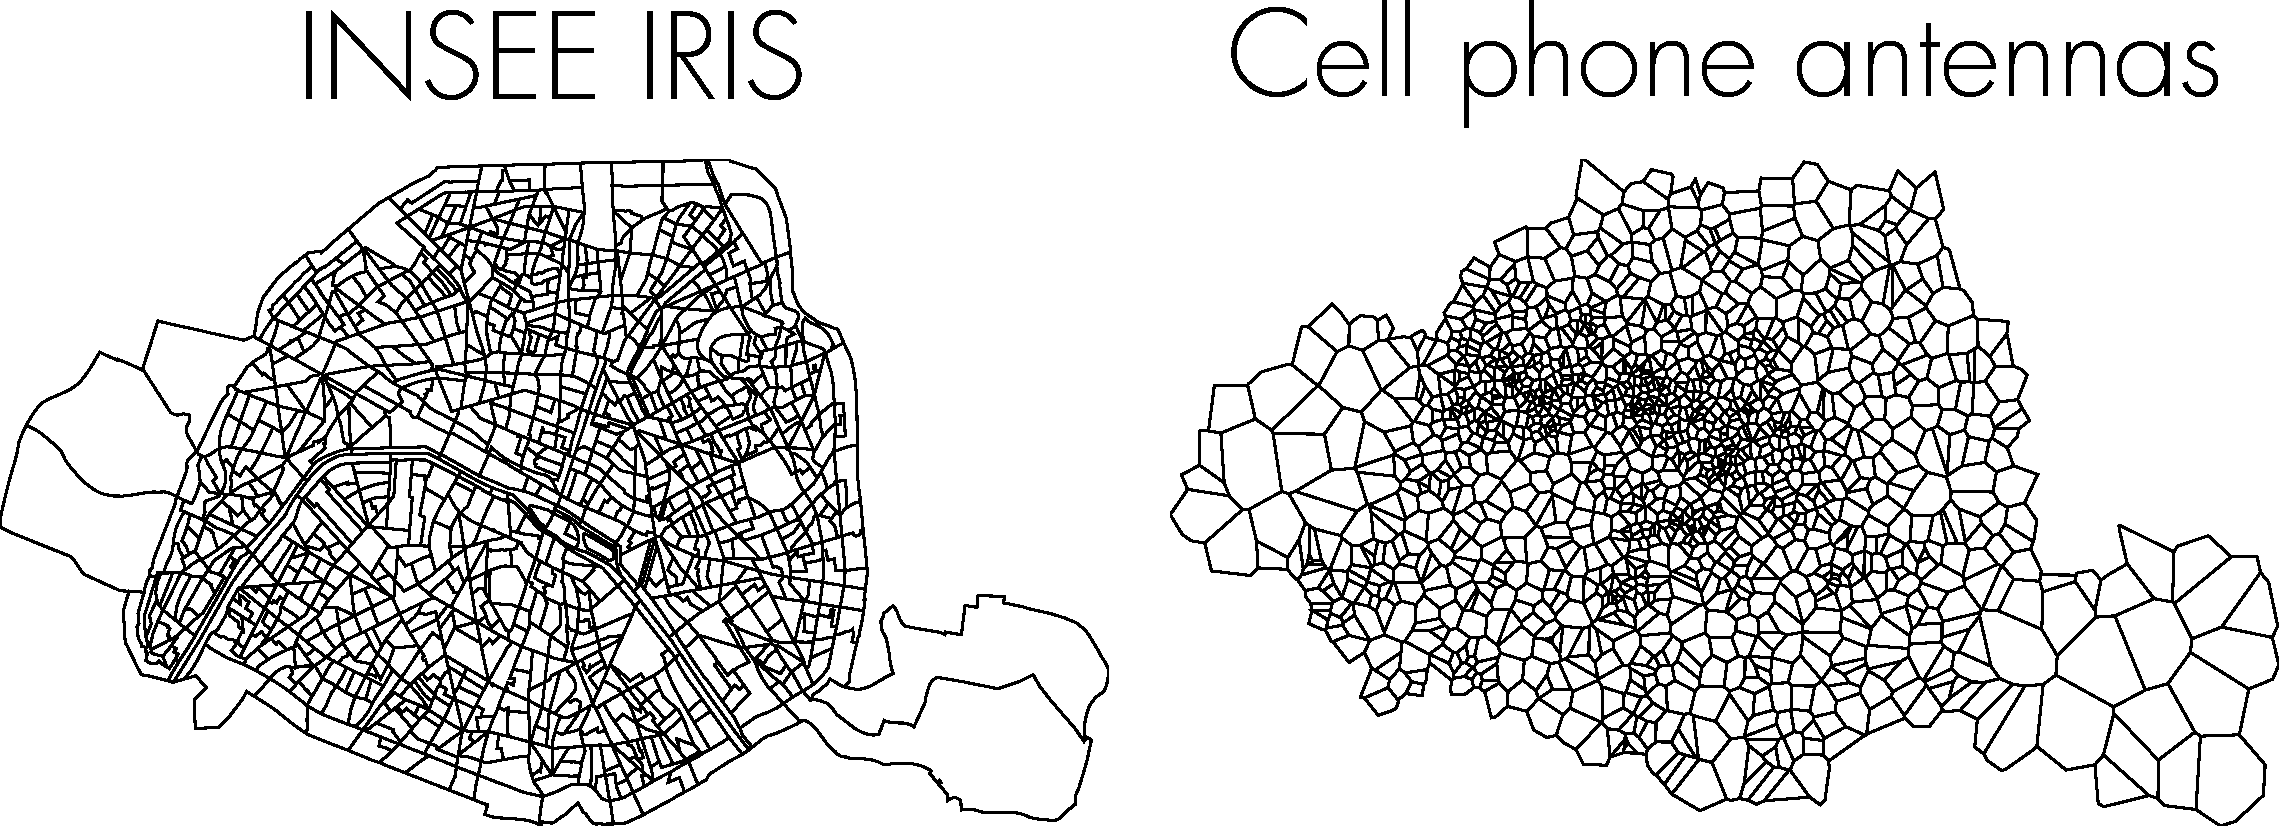
\includegraphics[width=\textwidth]{gfx/chapter-intro/IRIS_phone.pdf}
    \caption{(Left) IRIS zones in Paris, the smallest statistical units defined
    by the national statistics institute, INSEE. (Right) Voronoi tesselation
    built from the position of antennas of a popular french mobile phone carrier.
    There are $40\%$ more antennas than there are IRIS, and they tend to be more
    concentrated in zones of high daily activity (8th and 9th
    arrondissements).\label{fig:IRIS_phone}}
\end{figure}

Mobile phone data are spatially more precise. They give us a \emph{continuous}
information about the flow of individuals within the city, and not only
commuting.

But be careful. If they are ok to monitor aggregate quantities, be careful of
individuals trajectories because sampled in a weird way.

    \subsection{A technological convergence}
    \label{sub:a_technological_convergence} 

It is difficult to make a concise summary of what is known and not known about
urban systems. The vast amount of knowledge that has been gathered so far seems
very little in comparison to the bewildering complexity of the object being
studied~\cite{Batty:2008}. Every map, every satellite view, every statistic, every step
in cities elicits a question yet to be answered. What do we have to answer them?
A surprisingly small array of empirical tools and models. A surprisingly small
amount of solid, undisputed empirical facts.\\

This pessimistic account is not to belittle the previous contributions to the
field, however. They did what is the most difficult: laying the conceptual
ground on which detailed enquiries can flourish. One thing I have learned, not
through reading philosophy of science books, or casual articles about the
scientific practice, but because I have been stuck myself, is that the most
difficult problems are conceptual ones. It is impossible to define a city
quantitatively a city before you have formed---with words, possibly drawings---a
conceptual picture of what a city is. It is impossible to study segregation
before you have logically clarified what one means by segregation---in the
spirit of analytic philosophy. However quantitative, an investigation built upon
weak conceptual foundations is unlikely to go anywhere, or to say anything
substantial. I have often found myself running in circles, multiplying the
number of measures performed, before finally leaving the keyboard alone to lay
down my thoughts on paper. On the other hand, when the thoughts have settled and
the question is clear, one can quickly make a substantial contribution.\\

A lesson painstakingly learned during this thesis is that \emph{thinking} the
city is as important as \emph{measuring} the city, or \emph{modeling} the city.
Concepts guide us and tell us what to measure, what to model. In the same way
measures and model can tell us what to think. But it would be very naive to
believe that scientific enquiries are fueled by the sole discussion between
measures and models. A quick inspection of the literature reveals, in fact, that
many studies are based upon an intuition, a pattern that the author has felt and
whose existence she is trying to prove on a quantitative basis. They are based
on an hypothesis, an intuition, a vision. Something difficult to explain with
words, but that I am sure the reader will recognise in his own research
practice.
